\documentclass{examen}

\begin{document}
\modulo{Redes}
\pregunta{�Qu� significa que IP sea independiente de los medios? �y que sea un servicio de mejor intento?}{1}

\pregunta{Explica dos de las ventajas que supone dividir una red en subredes}{0.5}
\pregunta{Explica dos de los criterios que se pueden seguir para dividir una red en subredes}{0.5}
\pregunta{Si un equipo tiene la IP 45.28.84.101, su m�scara es 255.255.224.0 y su puerta de enlace es 45.28.84.254 �que har� si desea enviar un paquete al nodo con la IP 45.28.13.101? Explica por qu�.}{1}
\pregunta{Di todo lo que sepas sobre el NAT}{0.5}
\pregunta{Una empresa necesita crear 4 subredes llamadas A, B, C y D. La subred A tiene 43 equipos, la B tiene 88, la C tiene 39 y la D 126. El prefijo que les han asignado es 00000111.10000011.10001xxx.xxxxxxxx. Indica las direcciones de red, de difusi�n y la primera y la �ltima IP de cada subred en el caso de que se pueda conseguir lo que pide esta empresa}{1}
\pregunta{Explica de la manera m�s completa posible qu� es el NAT y como funciona.}{1}
\pregunta{Convierte esta IPv6 a formato resumido {\tt fe80:a000:0000:0000:a300:a200:0000:0000}}{0.5}
\pregunta{Di todo lo que sepas sobre estas direcciones:
\begin{itemize}
\item{225.1.2.141}
\item{161.84.43.15}
\end{itemize}
}{1}
\pregunta{Una empresa tiene varias sedes con 4 routers A, B, C, D Indica las IP, m�scaras y las rutas que habr� que poner en dichos routers A, B, C y D(incluye las m�tricas junto a la direcci�n de siguiente salto).}{3}

\begin{figure}[h]
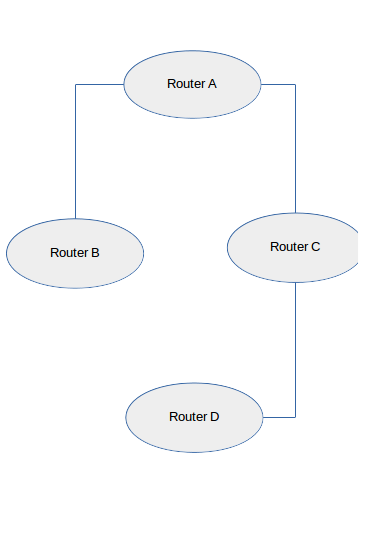
\includegraphics[scale=0.8]{examen-img/red_routers.png} 
\caption{Routers interconectados en red.}
\end{figure}


\end{document}
